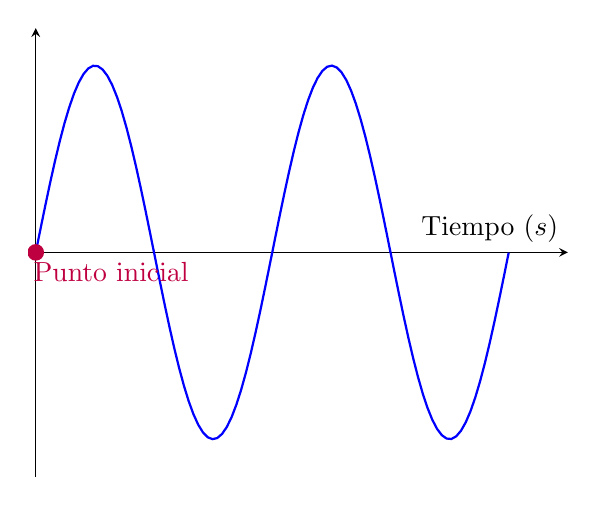
\begin{tikzpicture}
  \begin{axis}[
    xmin=-0.2,xmax=4.5*pi,
    ymin=-1.2,ymax=1.2,
    axis lines=middle,
    xtick={0},
    ytick={0},
    xlabel=Tiempo ($s$)
    ]

    % Funcion senoidal
    \addplot[color=blue,samples=100,domain=0:4*pi,thick]{sin(deg(x))};

    % Punto inicial
    \fill[purple] (axis cs:0,0) circle[radius=3pt];
    \node[purple,below] at (axis cs:2,0) {Punto inicial};
  \end{axis}
\end{tikzpicture}
